\subsection{Outline how the spin-orbit coupling arises. Discuss the resulting splitting of the energy states for the case of hydrogen.}


Vi kender et atom som havende en elektron i en cirkulær banebevægelse med hastihed $\Vec{v}$ rundt om en kerne af $Z$ partikler, ??? hvorfor elektronen både har et baneimpulsmoment samt spin ??? . Ses dette billede nu fra elektronens perspektiv, så er det kernen, som bevæger sig i en cirkulær banebevægelse med hastighed $\Vec{v}$ rundt om elektronen. Denne cirkelbevægelse af en positivt partikel resulterer i en cikulær strøm
\begin{align}
    \Vec{I} &= \rho \Vec{v} = - \frac{Z e}{2\pi r} \Vec{v} \: , \quad \rho: \: \text{strømtæthed}
\end{align}
som fra Biot-Savarts lov danner et magnetfelt, som ved elektronen er
\begin{align}
    \Vec{B}_l &= \frac{\mu_0 Z e}{4\pi r^3}\left(\Vec{v} \cross \left(-\Vec{r}\right)\right) = - \frac{\mu_0 Z e}{4\pi r^3}\left(\Vec{v} \cross \Vec{r}\right) = \frac{\mu_0 Z e}{4\pi m_e r^3}\Vec{l} \: ,
\end{align}

\begin{figure}[!h]
    \centering
    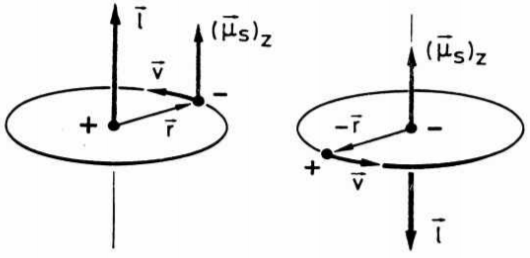
\includegraphics[width=0.75\textwidth]{Q10/images/SpinOrbiCouplingAtomFromDifferentPerspectives.PNG}
    \caption{Transformation fra kernens til elektronens perspektiv.}
    \label{fig:my_label}
\end{figure}